% Copyright (C) 2005-2015 Airbus - EDF - IMACS - Phimeca
% Permission is granted to copy, distribute and/or modify this document
% under the terms of the GNU Free Documentation License, Version 1.2
% or any later version published by the Free Software Foundation;
% with no Invariant Sections, no Front-Cover Texts, and no Back-Cover
% Texts.  A copy of the license is included in the section entitled "GNU
% Free Documentation License".
\renewcommand{\filename}{docUC_InputNoData_CompositeDistribution.tex}
\renewcommand{\filetitle}{UC : Creation  of 1D distribution from a 1D distribution}

% \HeaderNNIILevel
% \HeaderIILevel
\HeaderIIILevel





\index{Composed Distribution}


The objective of the Use Case is to create a distribution, defined as the push-forward distribution of a scalar distribution  by a transformation $\Rset \rightarrow \Rset$. \\

If we note $\mathcal{L}_0$ a scalar distribution, $f: \Rset \rightarrow \Rset$ a mapping, then OpenTURNS enables to easily create the push-forward distribution $\mathcal{L}$ defined by: 
\begin{align}
\mathcal{L} = f(\mathcal{L}_0)
\end{align}
which means that for all scalar random variable $X$ following the distribution $\mathcal{L}_0$, $Y=f(X)$ follows the distribution $\mathcal{L}$. \\

Note that for the following usual transformations $f$, a simplified notation has been implemented: \emph{cos, sin, tan, acos, asin, atan, cosh, sinh, tanh, acosh, asinh, atanh, exp,  log, ln, pow, inverse, sqr, sqrt, cbrt, abs}.  If the operators are chained, they are applied from left to right. See the foolowing script for some examples.


             \textspace\\

\noindent%
\requirements{
  \begin{description}
  \item[$\bullet$] a scalar distribution : {\itshape myAntecedentDist}
  \item[type:] Distribution
  \end{description}

  \begin{description}
  \item[$\bullet$] a mapping  $\Rset \rightarrow \Rset$: {\itshape f}
  \item[type:] NumericalMathFunction
  \end{description}
}
             {
  \begin{description}
  \item[$\bullet$] a scalar distribution : {\itshape myImageDist}
  \item[type:] CompositeDistribution
  \end{description}
             }

             \textspace\\
             Python script for this UseCase :

             \inputscript{script_docUC_InputNoData_CompositeDistribution}

             \textspace\\
The following figures illustrate the cases where $\mathcal{L}_0$ is the Normal() distribution and $f$ the function defined by:
\begin{itemize}
  \item  $f(x)=\sin(x) + \cos(x)$ in the figure  \ref{Imagedist};
  \item  $f(x)=\exp(x)$  in the figure   \ref{Imagedist2};
  \item  $f(x)=\sqrt{|x|}$  in the figure   \ref{Imagedist3}.
\end{itemize}




\begin{figure}[H]
  \begin{minipage}{9cm}
    \begin{center}
      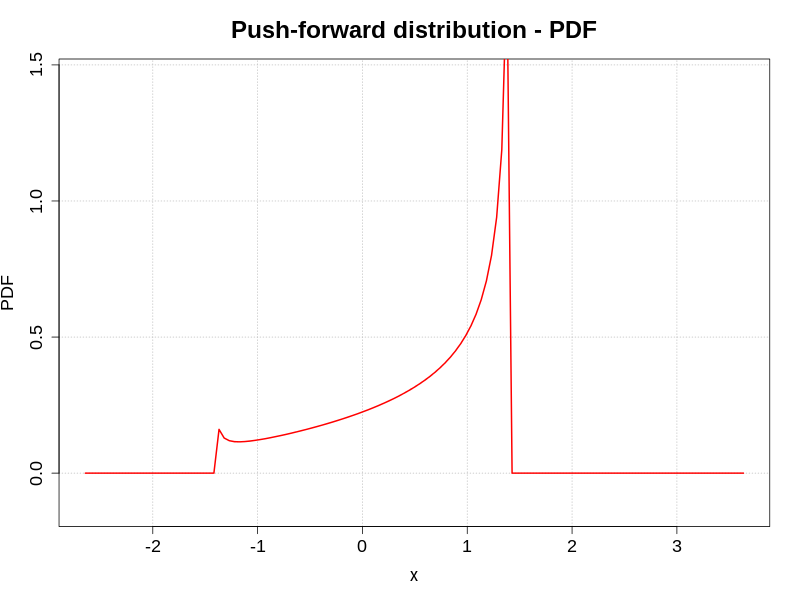
\includegraphics[width=7cm]{Figures/ImageDist.png}
      \caption{PDF of the push-forward distribution of a Normal() mapped through $f(x)=\sin(x) + \cos(x)$}
      \label{Imagedist}
    \end{center}
  \end{minipage}
  \hfill
  \begin{minipage}{9cm}
    \begin{center}
      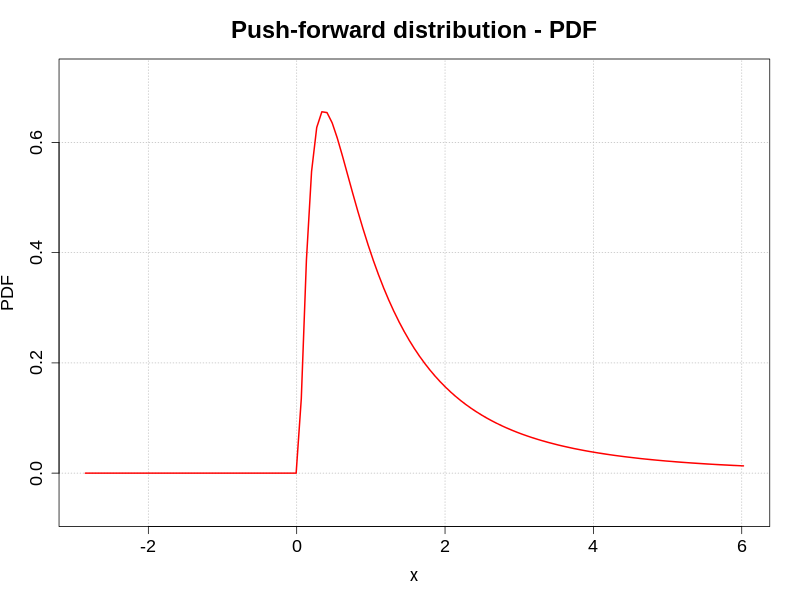
\includegraphics[width=7cm]{Figures/ImageDist2.png}
      \caption{PDF of the push-forward distribution of a Normal() mapped through $f(x)=\exp(x)$}
      \label{Imagedist2}
    \end{center}
  \end{minipage}
\end{figure}

\begin{figure}[H]
  \begin{center}
      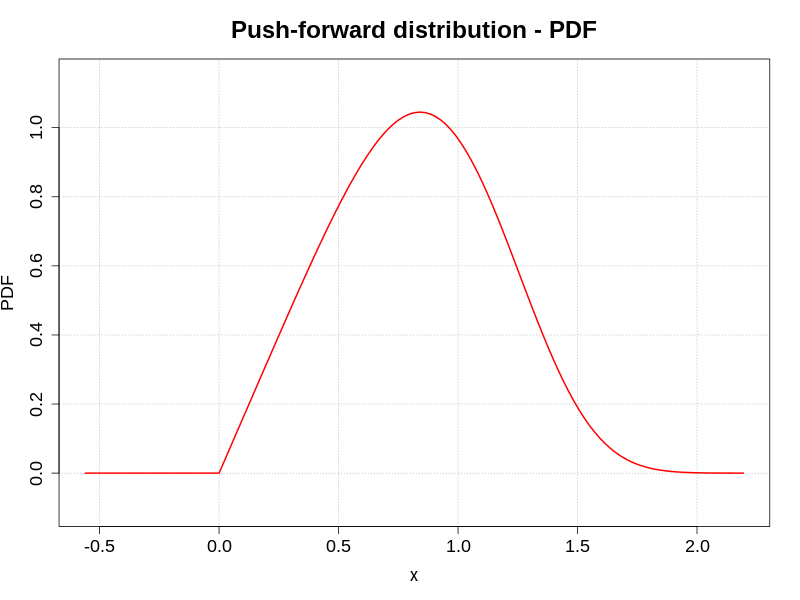
\includegraphics[width=7cm]{Figures/ImageDist3.png}
      \caption{PDF of the push-forward distribution of a Normal() mapped through $f(x)=\sqrt{|x|}$}
      \label{Imagedist3}
    \end{center}
\end{figure}
